q
\begin{figure}[h!]
	\centering{
		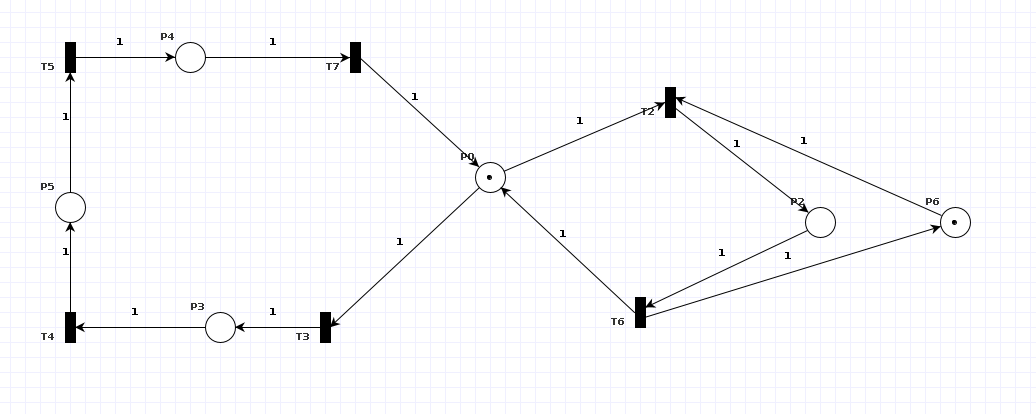
\includegraphics[width=0.67\textwidth]{img/2.png}
	}
	\caption{Sieć reprezentująca wzajemne używanie zasobów}
	\label{zad2:graph1}
\end{figure}
\begin{figure}[h!]
	\centering{
		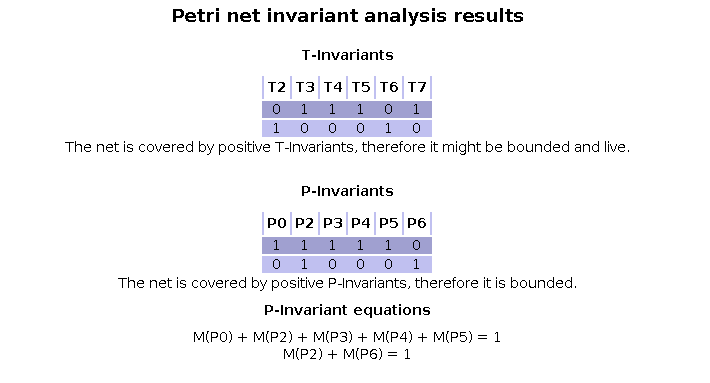
\includegraphics[width=0.75\textwidth]{img/kryt.png}
	}
	\caption{Niezmienniki sieci}
	\label{zad2:graph1}
\end{figure}

\subsection{Analiza niezminników sieci}
Równanie pierwsze chroni nam sekcję krytyczną. 

Równanie drugie wskazuje na to, że w każdym momencie dokładnie jeden z procesów 
po prawej stronie sieci jest uruchomiony.

